% ================= SEKCJA 10 =================
\section{Stos technologiczny}

Stos technologiczny systemu \texttt{WorkFlow} został dobrany w taki sposób, aby umożliwić stworzenie aplikacji webowej z wyraźnym podziałem na frontend, backend, bazę danych, magazyn plików oraz warstwę uruchomieniową. Przy wyborze technologii uwzględniono możliwość pracy w języku TypeScript, dostępność narzędzi wspierających szybkie tworzenie interfejsu, wygodną komunikację z bazą danych oraz możliwość uruchomienia całego systemu w kontenerach Docker.

Zastosowany zestaw technologii nie wymaga ręcznej instalacji wszystkich usług na komputerze użytkownika. Projekt został przygotowany tak, aby można było uruchomić środowisko za pomocą Docker Compose, co ułatwia testowanie, prezentację i dalszy rozwój aplikacji.

\begin{figure}[H]
    \centering
    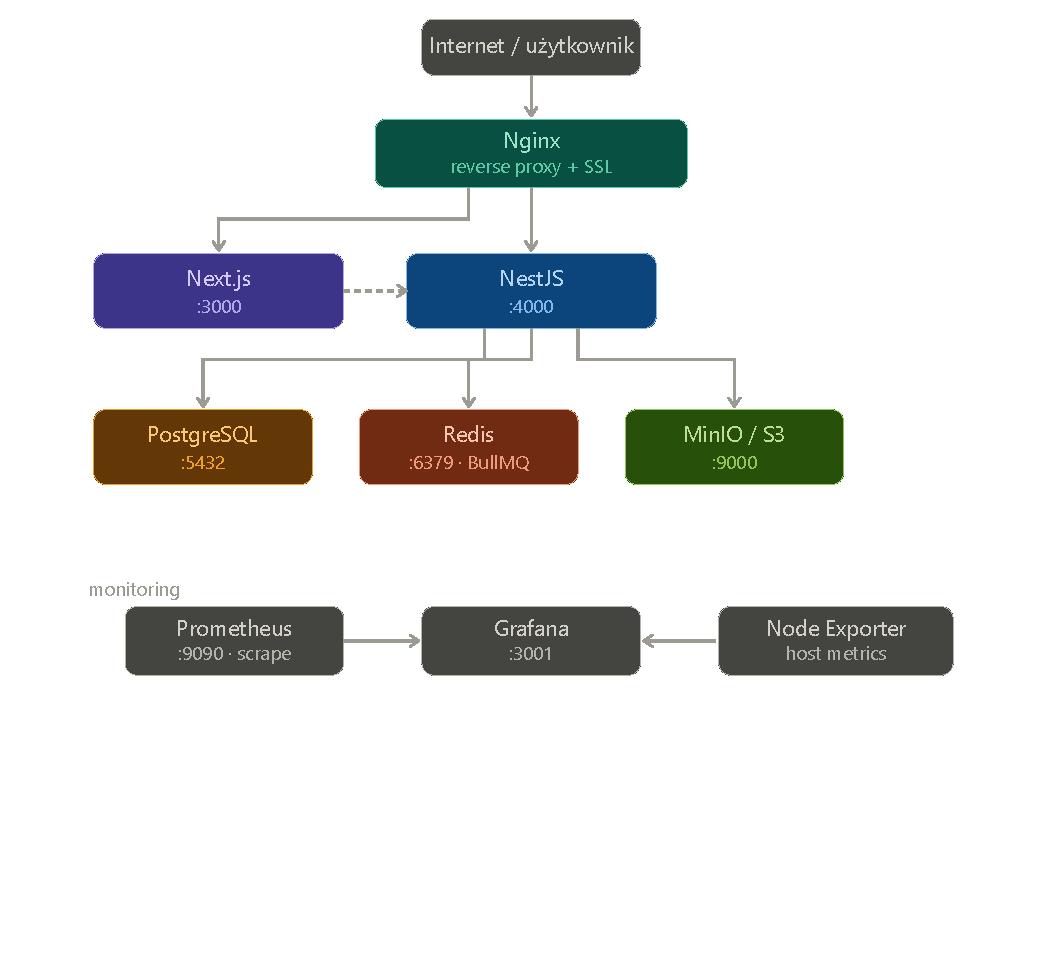
\includegraphics[width=0.85\textwidth]{rys/stack.pdf} 
    \caption{Stos technologiczny i podstawowa architektura systemu \texttt{WorkFlow}}
    \label{fig:deployment_arch}
\end{figure}

\subsection{Warstwa prezentacji}

Warstwa prezentacji odpowiada za interfejs użytkownika dostępny z poziomu przeglądarki internetowej. Jej zadaniem jest wyświetlanie danych, obsługa formularzy, komunikacja z backendem oraz zapewnienie użytkownikowi dostępu do modułów zgodnych z jego rolą.

\begin{itemize}
    \item \textbf{Next.js} -- framework oparty na React, wykorzystany do budowy aplikacji frontendowej. Zapewnia strukturę projektu, routing oraz mechanizmy potrzebne do tworzenia nowoczesnych aplikacji webowych.
    \item \textbf{React} -- biblioteka służąca do budowy interfejsu użytkownika w oparciu o komponenty.
    \item \textbf{TypeScript} -- język rozszerzający JavaScript o statyczne typowanie. Zastosowanie TypeScript ułatwia kontrolę struktur danych przekazywanych pomiędzy komponentami i akcjami aplikacji.
    \item \textbf{Tailwind CSS} -- narzędzie do stylowania interfejsu za pomocą klas narzędziowych. Umożliwia szybkie budowanie spójnych widoków bez konieczności tworzenia dużej liczby osobnych arkuszy CSS.
    \item \textbf{shadcn/ui} -- zestaw komponentów interfejsu użytkownika, wykorzystywany jako baza dla formularzy, przycisków, pól wyboru, tabel i innych elementów aplikacji.
    \item \textbf{TanStack Query} -- biblioteka wspierająca pobieranie i odświeżanie danych po stronie frontendu. Ułatwia obsługę stanów ładowania, błędów oraz ponownego pobierania danych.
\end{itemize}

W warstwie frontendowej istotne było również zachowanie spójności wyglądu w trybie jasnym i ciemnym. W tym celu interfejs został oparty na klasach i tokenach kolorystycznych, które pozwalają dostosować wygląd komponentów do aktywnego motywu.

\subsection{Warstwa logiki biznesowej}

Warstwa backendowa odpowiada za logikę biznesową systemu, obsługę API, autoryzację, walidację danych oraz komunikację z bazą danych i magazynem plików. Backend jest oddzielną usługą uruchamianą w kontenerze Docker.

\begin{itemize}
    \item \textbf{NestJS} -- framework backendowy dla Node.js, oparty na TypeScript. Umożliwia organizację kodu w moduły, kontrolery, serwisy i guardy, co ułatwia utrzymanie większej aplikacji.
    \item \textbf{Node.js} -- środowisko uruchomieniowe JavaScript wykorzystywane przez backend.
    \item \textbf{JWT} -- mechanizm tokenów wykorzystywany do autoryzacji użytkowników po zalogowaniu.
    \item \textbf{Guards w NestJS} -- mechanizmy służące do ochrony wybranych endpointów, sprawdzania tokenu użytkownika, roli oraz tokenu technicznego dla urządzeń RCP.
    \item \textbf{DTO i walidacja danych} -- struktury opisujące dane wejściowe API oraz walidujące poprawność żądań przed wykonaniem operacji biznesowej.
\end{itemize}

Backend udostępnia zarówno endpointy wykorzystywane przez frontend, jak i endpoint techniczny przeznaczony do odbierania zdarzeń z czytników RCP. Dzięki temu jedna warstwa logiki biznesowej obsługuje zarówno działania użytkowników, jak i zdarzenia pochodzące z urządzeń.

\subsection{Warstwa danych}

Dane systemu przechowywane są w relacyjnej bazie PostgreSQL. Baza danych zawiera tabele opisujące pracowników, zakłady, projekty, przypisania, umowy, certyfikaty, dokumenty, nieobecności, czas pracy, eksporty rozliczeniowe oraz wpisy audytowe.

\begin{itemize}
    \item \textbf{PostgreSQL} -- relacyjna baza danych wykorzystywana jako główne miejsce przechowywania danych systemu.
    \item \textbf{Prisma ORM} -- narzędzie pośredniczące pomiędzy backendem a bazą danych. Prisma pozwala definiować modele danych w pliku \texttt{schema.prisma} oraz wykonywać operacje na bazie z poziomu kodu TypeScript.
    \item \textbf{Prisma Client} -- wygenerowany klient wykorzystywany w kodzie backendu do komunikacji z bazą danych.
    \item \textbf{Prisma db push} -- polecenie używane do synchronizacji struktury bazy danych ze schematem Prisma.
\end{itemize}

Zastosowanie Prisma pozwala utrzymać model danych blisko kodu aplikacji. Dzięki temu łatwiej kontrolować relacje między encjami i zachować zgodność pomiędzy typami wykorzystywanymi w kodzie a strukturą bazy danych.

\subsection{Magazyn plików}

System przechowuje dokumenty pracowników poza relacyjną bazą danych. Do tego celu wykorzystano MinIO, czyli magazyn obiektowy kompatybilny z API S3.

\begin{itemize}
    \item \textbf{MinIO} -- usługa odpowiedzialna za przechowywanie plików dokumentów.
    \item \textbf{Bucket dokumentów} -- wydzielone miejsce w MinIO przeznaczone na pliki związane z pracownikami, umowami, certyfikatami i nieobecnościami.
    \item \textbf{Metadane dokumentów w PostgreSQL} -- baza danych przechowuje informacje o nazwie pliku, właścicielu dokumentu i ścieżce do pliku, natomiast sam plik znajduje się w magazynie obiektowym.
\end{itemize}

Oddzielenie plików od danych relacyjnych upraszcza model bazy danych i pozwala uniknąć przechowywania dużych plików bezpośrednio w tabelach.

\subsection{Warstwa infrastruktury}

Do uruchomienia systemu wykorzystano Docker oraz Docker Compose. Każda główna część aplikacji działa jako osobna usługa, dzięki czemu można jasno określić odpowiedzialność poszczególnych komponentów.

\begin{itemize}
    \item \textbf{Docker} -- technologia konteneryzacji umożliwiająca uruchamianie usług w izolowanych kontenerach.
    \item \textbf{Docker Compose} -- narzędzie służące do definiowania i uruchamiania wielu kontenerów jako jednego środowiska.
    \item \textbf{Nginx} -- reverse proxy kierujące ruch użytkownika do frontendu oraz zapytania API do backendu.
    \item \textbf{Plik \texttt{.env}} -- plik zawierający zmienne środowiskowe, takie jak hasła, tokeny, porty i adresy usług.
    \item \textbf{Plik \texttt{.env.example}} -- przykładowy plik konfiguracyjny przechowywany w repozytorium bez rzeczywistych sekretów.
\end{itemize}

W środowisku Docker Compose uruchamiane są następujące usługi:
\begin{itemize}
    \item frontend,
    \item backend,
    \item PostgreSQL,
    \item MinIO,
    \item Nginx.
\end{itemize}

Nginx upraszcza dostęp do aplikacji, ponieważ użytkownik korzysta z jednego adresu. Ruch do interfejsu użytkownika trafia do frontendu, natomiast ścieżki API są przekazywane do backendu.

\subsection{Seedowanie danych}

W projekcie przygotowano mechanizmy seedowania bazy danych. Ich zadaniem jest ułatwienie uruchomienia systemu oraz przygotowanie środowiska demonstracyjnego.

\begin{itemize}
    \item \textbf{Seed minimalny} -- tworzy podstawowe dane potrzebne do rozpoczęcia pracy, między innymi główny zakład oraz konta startowe dla ról administratora, HR, księgowości i brygadzisty.
    \item \textbf{Seed demonstracyjny} -- tworzy pełniejszy zestaw danych, obejmujący pracowników, projekty, czytniki RCP, umowy, certyfikaty, dokumenty, nieobecności, wpisy czasu pracy oraz przykładowy eksport rozliczeniowy.
\end{itemize}

Seed demonstracyjny jest szczególnie przydatny podczas prezentacji projektu, ponieważ pozwala pokazać działanie systemu bez ręcznego wprowadzania wszystkich danych. Ze względu na to, że może on czyścić istniejące dane, jego uruchomienie wymaga dodatkowego potwierdzenia przez zmienną środowiskową.

\subsection{Komunikacja pomiędzy usługami}

W środowisku kontenerowym poszczególne usługi komunikują się ze sobą za pomocą nazw usług zdefiniowanych w Docker Compose. Backend łączy się z bazą PostgreSQL, komunikuje się z MinIO oraz udostępnia API dla frontendu i czytników RCP.

Frontend komunikuje się z backendem przez adres API skonfigurowany w zmiennych środowiskowych. W środowisku uruchamianym przez Nginx zapytania API mogą być kierowane przez ścieżkę \texttt{/api}, co pozwala zachować jeden zewnętrzny adres aplikacji.

\subsection{Uzasadnienie wyboru technologii}

Wybrane technologie pozwalają utrzymać spójny stos oparty głównie na TypeScript. Frontend i backend korzystają z tego samego języka, co ułatwia pracę nad typami danych i strukturą kodu. PostgreSQL zapewnia stabilną bazę relacyjną, Prisma upraszcza komunikację z bazą, a MinIO pozwala oddzielić dokumenty od danych relacyjnych.

Docker Compose umożliwia uruchomienie kompletnego środowiska za pomocą jednej konfiguracji. Jest to istotne zarówno podczas lokalnego testowania, jak i podczas przygotowania projektu do prezentacji lub wdrożenia na serwerze.

Zastosowany stos technologiczny jest wystarczający do obsługi aktualnego zakresu systemu i jednocześnie pozostawia możliwość dalszej rozbudowy, na przykład o powiadomienia, dodatkowe raporty, integrację z systemem księgowym lub zewnętrznym dostawcą tożsamości.